\section{Limitations of the SQ framework}
\label{sec:limitations}
% \begin{enumerate}
%     \item write about parity functions and how they cannot be solved with SQ but can be solved with PAC (section 3.1.2)
%     \item Maybe section 3.3 of the paper fits more here
% \end{enumerate}

\subsection{Classes that are not efficiently SQ learnable}
Using the statistical query dimension, the lower bounds, and Corollary \ref{not_learnable}, we can now look at some functions that are not learnable using statistical queries.

\begin{proposition}
\label{parity_fn}
Parity functions $f: \{-1, 1\}^n \xrightarrow{} \{-1, 1\}$ have SQ-DIM $= 2^n$, and therefore, are not efficiently SQ learnable.
\end{proposition}

Parity functions can be given as $f(x) = \prod_{i \in [n]} x_i$. All $2^n$ of these are pairwise orthogonal (\cite{odonnell_analysis_2014}), therefore their SQ dimension is also $2^n$. Thus, according to Corollary \ref{not_learnable} we know they are not efficiently SQ learnable.

\cite{blum_noise-tolerant_2003} extend this and show that parity functions with some constraints are efficiently PAC learnable in the presence of random classification noise.

\begin{proposition}
Decision trees with $n$ nodes have SQ-DIM $\geq n^{c.log(n)}$, and therefore, are not efficiently SQ learnable.
\end{proposition}

Decision trees can be encoded by parity functions and as shown in Preposition \ref{parity_fn} parity functions are not efficiently SQ learnable, thus, so are decision trees.

A decision tree with $n-1$ nodes can be encoded by a parity function of size $log(n)$ as shown in Figure \ref{fig:decision_tree}. Since there are $^nC_{logn(n)}$ choices to choose $log(n)$ from $n$ variables, this shows that decision trees have statistical query dimension of at least $n^{c.log(n)}$.

\begin{figure*}
    \centering
    \subfigure[]{
        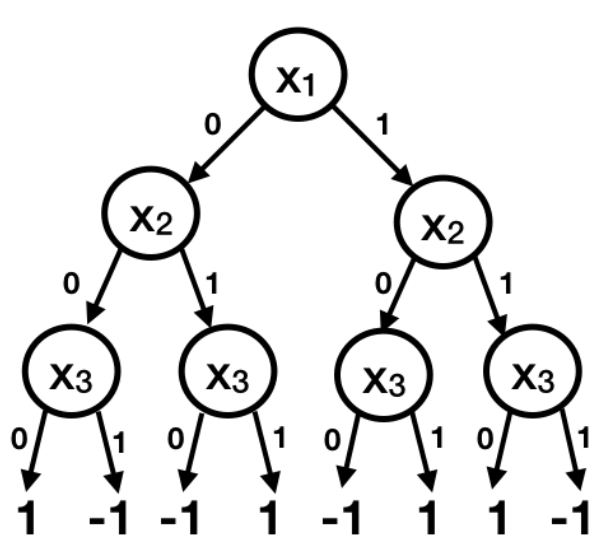
\includegraphics[width=0.25\textwidth]{report/figs/decision_tree.png}
        \label{fig:decision_tree}
    }
    \subfigure[]{
        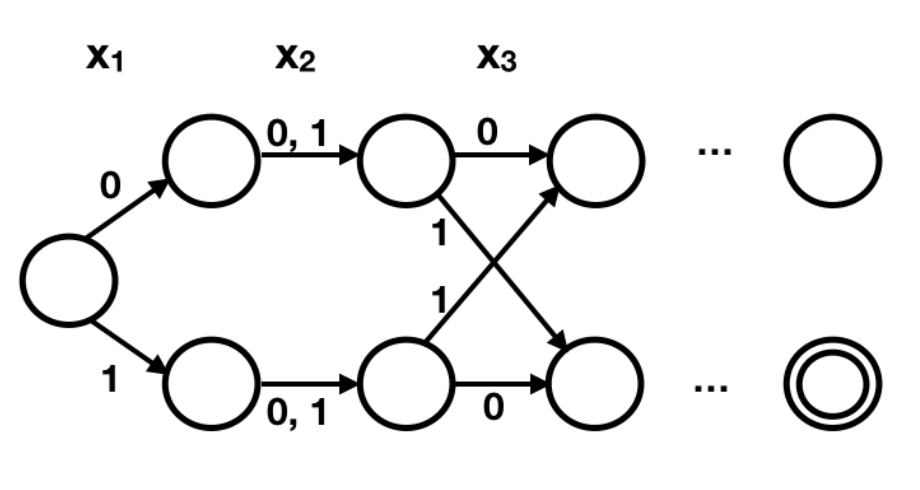
\includegraphics[width=0.4\textwidth]{report/figs/dfa.png}
        \label{fig:dfa}
    }
    \caption{(a) A decision tree with $7$ nodes encoding a parity function of size $3$ (b) A deterministic finite automata with $2n + 1$ nodes encoding a parity function of size $n$}
\end{figure*}
 
% \begin{figure}
%     \centering
%     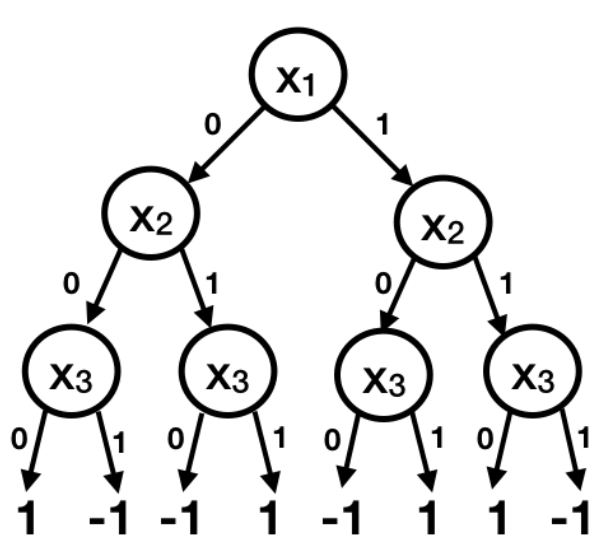
\includegraphics[width=0.4\textwidth]{report/figs/decision_tree.png}
%     \caption{A decision tree with $7$ nodes encoding a parity function of size $3$}
%     \label{fig:decision_tree}
% \end{figure}

\begin{proposition}
Disjunctive normal form (DNF) expressions of size $n$ have SQ-DIM $\geq n^{c.log(n)}$, and therefore, are not efficiently SQ learnable.
\end{proposition}

Like decision trees, DNF formulae can also be encoded by parity functions. The following is a $4$-term DNF encoded by a parity function of size $3$.
\begin{align*}
    (x_1 \wedge x_2 \wedge x_3) \vee (\overline{x_1} \wedge \overline{x_2} \wedge \overline{x_3}) \vee (\overline{x_1} \wedge x_2 \wedge \overline{x_3}) \vee (\overline{x_1} \wedge \overline{x_2} \wedge x_3)
\end{align*}

\begin{proposition}
Deterministic finite automata with $n$ nodes have SQ-DIM $\geq 2^{c.n}$, and therefore, are not efficiently SQ learnable.
\end{proposition}

As shown in Figure \ref{fig:dfa}, deterministic finite automata with $2n+1$ nodes can also encode a parity function of size $n$.

% \begin{figure}
%     \centering
%     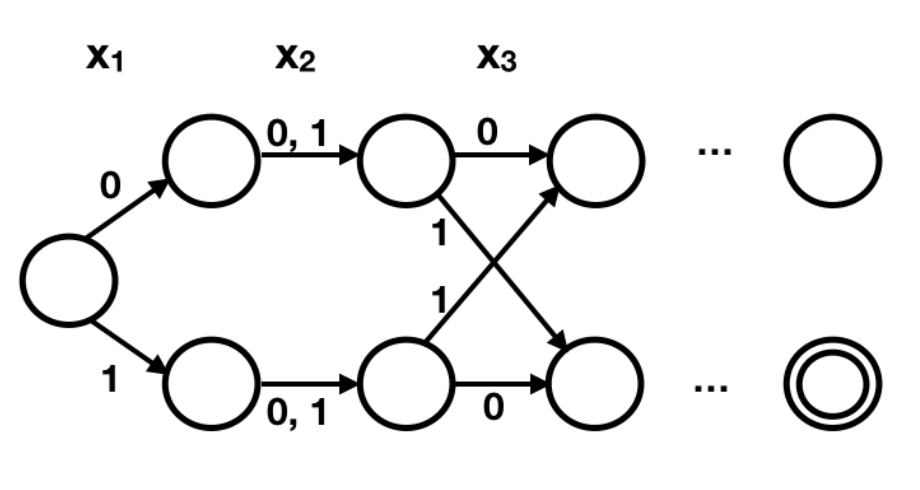
\includegraphics[width=0.4\textwidth]{report/figs/dfa.png}
%     \caption{A deterministic finite automata with $2n + 1$ nodes encoding a parity function of size $n$}
%     \label{fig:dfa}
% \end{figure}

\subsection{Complexity of learning}
Based on the above discussion, we can write the following hierarchy of models that contain the classes of functions that are learnable in those respective models:
\begin{align*}
    \text{efficient SQ} \subseteq \text{efficient PAC under classification noise} \subseteq \text{efficient PAC}
\end{align*}
